\documentclass[border=10pt]{standalone}
\usepackage{pgfplots}
\pgfplotsset{compat=1.18}
\begin{document}
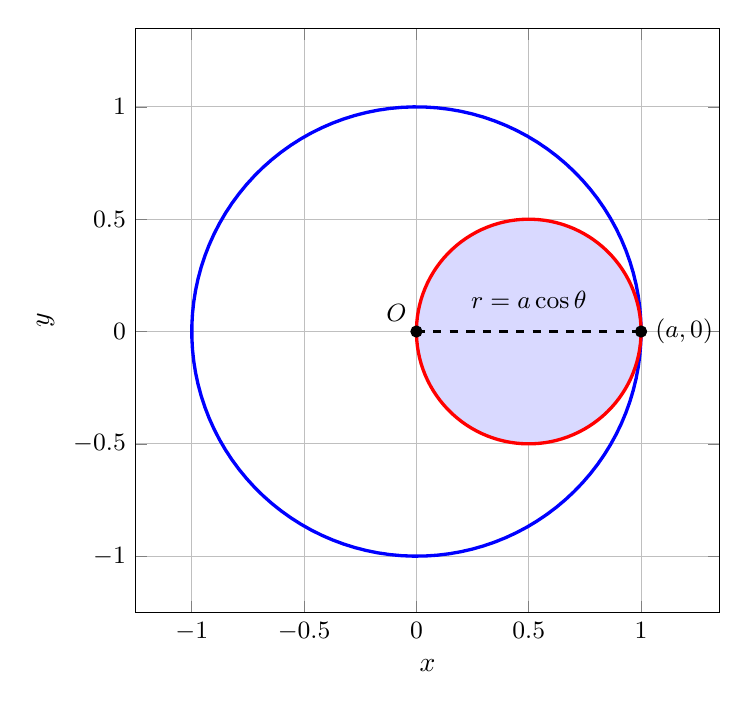
\begin{tikzpicture}
\begin{axis}[
    axis equal,
    xmin=-1.25, xmax=1.35,
    ymin=-1.25, ymax=1.35,
    xlabel=$x$, ylabel=$y$,
    width=9cm, height=9cm,
    grid=major,
    tick label style={font=\small},
]
% Shade the projection D = cylinder disk
\addplot[fill=blue!15, draw=none, domain=-90:90, samples=120]
    ({cos(x)^2}, {cos(x)*sin(x)}) -- cycle;

% Sphere projection circle
\addplot[blue, very thick, domain=0:360, samples=120]
    ({cos(x)}, {sin(x)});

% Cylinder circle
\addplot[red, very thick, domain=0:360, samples=120]
    ({0.5+0.5*cos(x)}, {0.5*sin(x)});

% Radial segment from O to (a,0)
\addplot[black, dashed, thick, domain=0:1, samples=2] ({x}, {0});

% Points O and (a,0)
\addplot[only marks, mark=*, mark size=2pt, color=black] coordinates {(0,0) (1,0)};

\node[anchor=south, font=\small] at (axis cs:0.5,0.06) {$r=a\cos\theta$};
\node[anchor=west, font=\small] at (axis cs:1+0.02,0) {$(a,0)$};
\node[anchor=south east, font=\small] at (axis cs:0,0) {$O$};
\end{axis}
\end{tikzpicture}
\end{document}
